
%(BEGIN_QUESTION)
% Copyright 2005, Tony R. Kuphaldt, released under the Creative Commons Attribution License (v 1.0)
% This means you may do almost anything with this work of mine, so long as you give me proper credit

Examine this three-phase motor control circuit (sometimes referred to as a ``bucket''), where fuses protect against overcurrent faults, a three-pole relay (called a {\it contactor}) turns power on and off to the motor, and a set of overload heaters detect mild overcurrent conditions.  Control circuit wiring has been omitted for simplicity's sake.  Only the power wiring is shown:

$$\includegraphics[width=15.5cm]{i01445x01.eps}$$

After years of faithful service, one day this motor refuses to start.  It makes a ``humming'' sound when the contactor is energized (relay contacts close), but it does not turn.  A mechanic checks it out and determines that the shaft is not seized, but is free to turn.  The problem must be electrical in nature!

You are called to investigate.  Using a clamp-on ammeter, you measure the current through each of the lines (immediately after each fuse) as another start is once again attempted.  You then record the three current measurements:

% No blank lines allowed between lines of an \halign structure!
% I use comments (%) instead, so that TeX doesn't choke.

$$\vbox{\offinterlineskip
\halign{\strut
\vrule \quad\hfil # \ \hfil & 
\vrule \quad\hfil # \ \hfil \vrule \cr
\noalign{\hrule}
%
% First row
Line & Current \cr
%
\noalign{\hrule}
%
% Another row
1 & 52.7 amps \cr
%
\noalign{\hrule}
%
% Another row
2 & 51.9 amps \cr
%
\noalign{\hrule}
%
% Another row
3 & 0 amps \cr
%
\noalign{\hrule}
} % End of \halign 
}$$ % End of \vbox

Determine at least two possible faults, either one fully capable of causing the motor's refusal to start and the three current measurements taken.  Then, decide what your next measurement(s) will be to isolate the exact location and nature of the fault.

\vskip 20pt \vbox{\hrule \hbox{\strut \vrule{} {\bf Suggestions for Socratic discussion} \vrule} \hrule}

\begin{itemize}
\item{} Is there a way we could have determined a lack of current in line 3 without the use of a clamp-on ammeter, using a multimeter incapable of directly measuring current over 10 amps?
\end{itemize}

\underbar{file i01445}
%(END_QUESTION)





%(BEGIN_ANSWER)

Here are some possibilities:

\begin{itemize}
\item{} Fuse \#3 blown open
\item{} Third relay contact damaged (failed open) inside the contactor
\item{} Overload heater \#3 failed open
\item{} One winding failed open inside the motor (assuming a ``Y'' winding configuration)
\end{itemize}

There are several valid ``next steps'' you could take from this point.  Discuss alternatives with your classmates.

%(END_ANSWER)





%(BEGIN_NOTES)

The fact that the motor hums but does not turn, along with the total lack of current through one line conductor, tells us the motor is being {\it single-phased}.

%INDEX% Electric motor (ORIGINAL GRAPHIC IMAGE FOR LIBRARY OBJECT)
%INDEX% Final Control Elements, motor: troubleshooting

%(END_NOTES)


